%
% Diagrama de la jerarquía de clases de un juego (ejemplo de herencia)
% Rubén Rubio (Universidad Complutense de Madrid) 2023
%

\documentclass[12pt, border=10pt]{standalone}

\usepackage[school]{pgf-umlcd}
\usepackage{fullpage}
\usepackage{fontspec}
\setmainfont{Source Sans 3}

\newcommand\attrcolor{\color{violet}}

\begin{document}
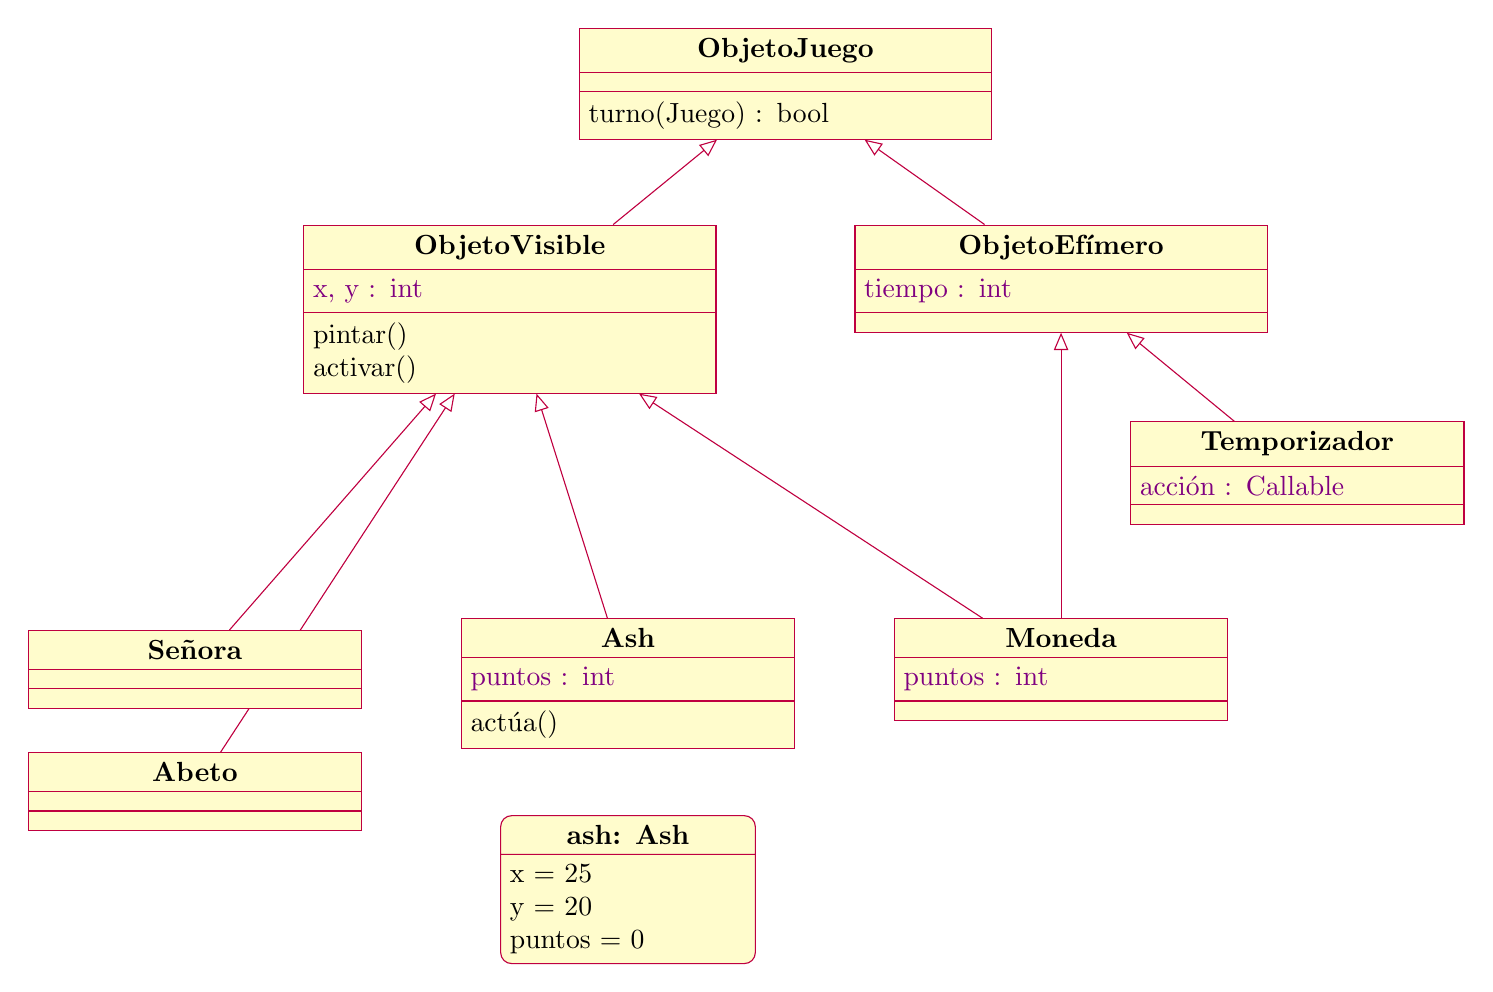
\begin{tikzpicture}

\begin{class}[text width=5cm]{ObjetoJuego}{0,0}
\operation{turno(Juego) : bool}
\end{class}

\begin{class}[text width=5cm]{ObjetoVisible}{-3.5,-2.5}
\inherit{ObjetoJuego}
\attribute{\attrcolor x, y : int}
\operation{pintar()}
\operation{activar()}
\end{class}

\begin{class}[text width=5cm]{ObjetoEfímero}{3.5,-2.5}
\inherit{ObjetoJuego}
\attribute{\attrcolor tiempo : int}
\end{class}

\begin{class}[text width=4cm]{Temporizador}{6.5,-5}
\inherit{ObjetoEfímero}
\attribute{\attrcolor acción : Callable}
\end{class}

\begin{class}[text width=4cm]{Ash}{-2,-7.5}
\inherit{ObjetoVisible}
\attribute{\attrcolor puntos : int}
\operation{actúa()}
\end{class}

\begin{object}[text width=3cm]{ash}{-2,-10}
\instanceOf{Ash}
\attribute{x = 25}
\attribute{y = 20}
\attribute{puntos = 0}
\end{object}

\begin{class}[text width=4cm]{Señora}{-7.5,-7.65}
\inherit{ObjetoVisible}
\end{class}

\begin{class}[text width=4cm]{Abeto}{-7.5,-9.2}
\inherit{ObjetoVisible}
\end{class}

\begin{class}[text width=4cm]{Moneda}{3.5,-7.5}
\inherit{ObjetoEfímero}
\inherit{ObjetoVisible}
\attribute{\attrcolor puntos : int}
\end{class}
\end{tikzpicture}
\end{document}
